\documentclass[a4paper,12pt]{article}
\usepackage{fullpage}
\usepackage{graphicx}

\setlength{\parindent}{0pt}

\def\pig{{\tt pig}}

\title{\pig, the PAG interface generator}
\author{Gerg\H{o} B\'ar\'any}

\begin{document}
\maketitle

\section{Introduction}
\pig\ is the PAG interface generator; it is a tool for automatical
generation of large parts of the glue code between a compiler front
end and PAG, the program analyzer generator.

More precisely, \pig\ is designed to generate the AST access
functions required by PAG (these are the \verb+is_op+ functions for
type tests, the \verb+get+ functions for child access, and several
functions for syntactic list traversal). Due to its flexible
specification language, \pig\ can also be used to generate such
access functions for other applications.

\pig\ is specialized for AST access since, given a well-designed
AST, most such accesses share a common structure and only differ in
details such as the names of the fields to be accessed or types to
be compared. This structure and the fact that many such functions
must be present suggest an automated approach to code creation.
In contrast, \pig\ cannot be utilized for generating the CFG access
functions, as each of these functions is unique and looks different
from the others.

The following sections describe in detail how \pig\ operates and how
you can operate it.

\section{Input and output}

The input to \pig\ consists of two files, one specifying the
abstract syntax and one containing macro rules describing the
functions to be created. It generates a C header and a code file.
This is sketched in Figure 1 below.

\begin{figure}
\begin{center}
\includegraphics{pig-diagram.ps}
\caption{Inputs and outputs of {\tt pig}}
\end{center}
\end{figure}

The first input file is called the {\em syn file}. It should be
identical to the \verb+syn+ file required by PAG. Thus, it contains
a tree grammar describing the structure of the abstract syntax trees
for which code is to be generated. It may also contain equations
declaring alias types; these are ignored by \pig. The syntax of the
syn file is not described further, you can find a description in the
PAG manual.

The other input file is the {\em spec file}. It contains rules that
describe which functions to create and how to create them. This is
the file against which all identifiers in the syn file are matched;
its syntax and the semantics of the matching and code generation are
described in the following section.

The names of the syn and spec files may be chosen freely, they are
passed to \pig\ on the command line.

The output files are called \verb+syntree.h+ and \verb+syntree.c+
as required by~PAG. The header file contains prototypes for all
functions generated by \pig\ or alternatively the macro definitions
for the functions that are to be implemented as macros. The code
file contains the definitions of the real functions specified by the
user. Additionally, \pig\ can add user-defined pre- and postfixes to
both files. This is useful for \verb+#include+ statements,
\verb+typedefs+, auxiliary functions and the like.

\section{Spec file syntax}

The syntax of the spec file is given below in an EBNF-like notation,
using [] for options, \(|\) for alternatives, and \(^*\) for zero or
more repetitions. Nonterminals are typeset in {\em italics},
terminal symbols in {\tt typewriter type}. Additional tokens are
{\em Code} for C code fragments, anything (except \verb+%}+)
enclosed in \verb+%{+ and \verb+%}+; {\em Id} for an identifier,
either a single \verb+_+ or a letter followed by any number of
letters, digits, or \verb+_+; {\em Str} for a string, an identifier
enclosed between \verb+"+; and {\em Num} for a number, a non-empty
sequence of digits.

Whitespace and comments (the usual types with \verb+//+ and
\verb+/*+ \ldots\ \verb+*/+) may be inserted anywhere between
tokens.

\begin{center}
\begin{tabular}{l c l}
{\em spec}     & ::= & {\em Code Code section\(^*\) Code Code} \\
{\em section}  & ::= & \verb+%%+ {\em keywords head body\(^*\)} \\
{\em keywords} & ::= & [\verb+per_constructor+] [\verb+list+] [\verb+macro+] \\
{\em head}     & ::= & {\em Id} \verb+:+ \verb+head+ \verb+(+{\em Id}\verb+,+
        {\em Id}\verb+,+ {\em Id}\verb+,+ {\em Id}\verb+,+ {\em
        Id}\verb+,+ {\em Id}\verb+,+ {\em Id}\verb+)+ {\em Code} \\
{\em body}     & ::= & {\em Id} \verb+:+ \verb+body+ \verb+(+{\em Id}\verb+,+
        {\em idstr}\verb+,+ {\em idstr}\verb+,+ {\em idnum}\verb+,+
        {\em idstr}\verb+,+ {\em idnum}\verb+,+ {\em idstr}\verb+)+
        {\em Code} \\
{\em idstr}    & ::= & {\em Id} \(|\) {\em Str} \\
{\em idnum}    & ::= & {\em Id} \(|\) {\em Num} \\
\end{tabular}
\end{center}

Each section is assigned a name, the identifier in front of the
\verb+head+ keyword. Each \verb+body+ rule in that section must be
assigned the same name.

Inside the argument lists of head and body rules, the identifiers
play the role of variable names, while strings and numbers are
constants. These argument lists are used for matching identifiers
from the syn file to rules in the spec file, as described in the
following section.

\section{Rule matching and the spec file}

The syn file consists of productions of the following form:

\begin{quote}
\begin{tabular}{r @{} c l}
{\em type} & {\tt:} & {\em constructor}{\verb+(+}{\em field}{\tt:}
        {\em field type}{\tt,} \ldots {\tt,}{ \em field}{\tt:}
        {\em field type}{\verb+)+} \\
 & \(\vdots\) & \\
 & {\tt|} & {\em constructor}{\verb+(+}{\em field}{\tt:}
        {\em field type}{\tt,} \ldots {\tt,}{ \em field}{\tt:}
        {\em field type}{\verb+)+} \\
 & {\tt;} & \\
\end{tabular}
\end{quote}

\pig's matcher traverses all such productions, and for each field
occurring in each production's alternatives, it creates a tuple
\begin{quote}
\em(type, constructor, constructor index, field, field index,
        field type).
\end{quote}

The constructor index is \(j\) for the \(j\)-th constructor for this
type, the field index is \(i\) for the \(i\)-th field for the
current constructor. Both are counted from~0.

The spec file is divided into sections, each of which describes one
function or macro to be implemented. A section consists of several
rules. The first rule in the section, called the {\em head} rule,
describes the function's prototype (or macro head), the other rules
are {\em body} rules describing possible implementations of the
function.

Each body rule is associated with an argument list whose members
(except the first one, which is ignored in matching) correspond to
the members of the tuples created from the syn file as described
above; these can be variables or constants of the appropriate type
(C identifiers for the type, constructor, field, and field type;
nonnegative integers for the indices).

The tuples from the syn files are matched against these rules: A
variable matches anything, a constant matches an identical constant.
In particular, an argument list containing only variables will match
every tuple. \pig\ chooses the first body rule matching the
constants from the syn file. The head and this body are then pasted
together and all variables instantiated with the constants; the
result is a function or macro definition that is emitted into the
output files.

Variable substitution is performed by the C preprocessor whose
\verb+##+ operator can also be used to paste tokens together.

The semantics of the three keywords are the following: The
\verb+per_constructor+ keyword means that the function defined in
this section should not be instatiated for every field but only once
for each constructor. This is necessary for functions that do not
depend on the field, for instance the \verb+is_op+ functions
required by PAG. If \verb+per_constructor+ were not used, \pig\
would emit several identical function definitions, causing problems
at compile time.

\verb+list+ means that the section should only be instantiated for
list fields, i.e. ones marked with \verb+*+ in the syn file. This is
used for list traversal functions such as \verb+empty+, \verb+hd+
and \verb+tl+. Implemententing such functions for non-list types
would not make sense.

Finally, \verb+macro+ instructs \pig\ to create the definitions for
this section not as functions but as C preprocessor macros.

\section{An example}

These theoretical explanations are best illustrated by an example.
Consider the following fictitious fragment of a syn file:

\begin{quote}
\begin{verbatim}
Statement: Assign(left: Var, right: Expr)
         | Loop(cond: Expr)
         ;
Expr     : Binary(left: Expr, right: Expr)
         | Unary(child: Expr)
         ;
\end{verbatim}
\end{quote}

Let us assume that the fields of a \verb+Statement+ node are to be
accessed by indexing an array of pointers, while the children of
\verb+Expr+s are accessed by name. Type information for the
\verb+is_op+ functions is stored in an enumeration. Additionally,
the \verb+get+ functions should be implemented as macros to avoid
the overhead of function calls.

The spec file might look like this:

\begin{quote}
\begin{verbatim}
%{ // prefix of syntree.c
#include "syntree.h"
%}

%% // section get
macro get:head(NODE, TYPE, CONSTR, _, FIELD, FIELDI, FTYPE)
%{
TYPE##_##CONSTR##_get_##FIELD(NODE)
%}

get:body(NODE, "Statement", _, _, _, FIELDI, _)
%{
    (NODE->children[FIELDI])
%}
get:body(NODE, "Expr", _, _, FIELD, _, _)
%{
    (NODE->FIELD)
%}

%% // section is_op
per_constructor is:head(NODE, TYPE, CONSTR, _, _, _, _)
%{
int is_op_##TYPE##_##CONSTR(TYPE NODE)
%}

is:body(NODE, _, CONSTR, _, _, _, _)
%{
    return (NODE->type == T_##CONSTR);
%}

%{%} // empty postfixes for syntree.h and syntree.c
%{%}
\end{verbatim}
\end{quote}

Given these inputs, \pig\ produces two files, \verb+syntree.h+ and
\verb+syntree.c+. The contents of \verb+syntree.h+ are the
following:

\begin{quote}
\begin{verbatim}
 // prefix of syntree.h
#include "type_definitions.h"

 #define Statement_Assign_get_left(NODE) (NODE->children[0])
int is_op_Statement_Assign(Statement NODE);
 #define Statement_Assign_get_right(NODE) (NODE->children[1])
 #define Statement_Loop_get_cond(NODE) (NODE->children[0])
int is_op_Statement_Loop(Statement NODE);
 #define Expr_Binary_get_left(NODE) (NODE->left)
int is_op_Expr_Binary(Expr NODE);
 #define Expr_Binary_get_right(NODE) (NODE->right)
 #define Expr_Unary_get_child(NODE) (NODE->child)
int is_op_Expr_Unary(Expr NODE);
\end{verbatim}
\end{quote}

Note that the \verb+#define+ statements are intermixed with function
prototypes. The reason for this is that \pig\ emits definitions
grouped by the fields defined in the syn file rather than by the
sections of the spec file. Observe also how the \verb+##+ operator
is used to create single tokens such as \verb+is_op_Expr_Binary+ out
of multiple parts and macros.

The \verb+syntree.c+ file looks like this (slightly reformatted to
fit the page):

\begin{quote}
\begin{verbatim}
 // prefix of syntree.c
#include "syntree.h"

int is_op_Statement_Assign(Statement NODE)
    { return (NODE->type == T_Assign);}
int is_op_Statement_Loop(Statement NODE)
    { return (NODE->type == T_Loop);}
int is_op_Expr_Binary(Expr NODE){ return (NODE->type == T_Binary);}
int is_op_Expr_Unary(Expr NODE){ return (NODE->type == T_Unary);}
\end{verbatim}
\end{quote}

The function definitions are completely expanded; this can be
requested with a flag passed to \pig. The default behavior is to
only emit a macro definition for each function and macro invocations
for each concrete function to be defined. This is a little more
compact and might be more readable under certain circumstances.

In this small example, the specification for \pig\ is longer than
the generated code. In real-world applications, however, the syn
file is considerably larger than in this case, causing much more
code to be emitted. Additionally, having a simple specification all
function definitions adhere to will often ease debugging,
maintenance and the addition of new features.

\end{document}
